\usetikzlibrary{calc,positioning,shapes,decorations.pathreplacing}

% the styles for short and long nodes
\tikzset{
short/.style={draw,rectangle,minimum height=1.5cm,
  text width=7pt,align=center,fill=gray!30, text centered},
long/.style={short,text width=1.9cm}
}

% the short nodes \shnode{<label>}{<right of>}{<text>}
\def\shnode#1#2#3{%
  \node[short,right=of #1] (#2) {\rotatebox{270}{#3}}}

% the long nodes \lnode{<label>}{<right of>}
\def\lnode#1#2#3#4{%
  \node[long,right=of #1,label={below:#4}] (#2) {#3}}
  
 \def\idnode#1#2#3#4{%
  \node[short,right=of #1,label={below:#4},style={short,text width=1.1cm}] (#2) {#3}}

\noindent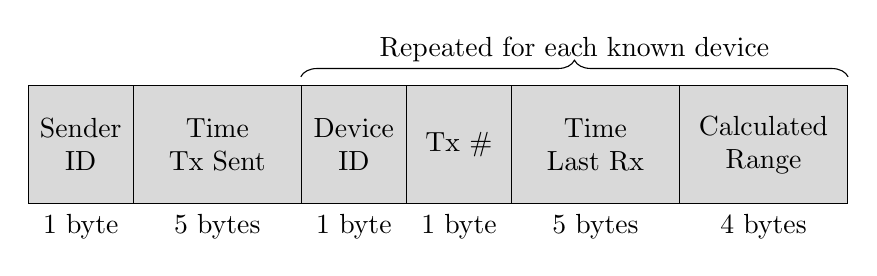
\begin{tikzpicture}[node distance=-\pgflinewidth]

\node[short,label={below:1 byte},style={short,text width=1.1cm}] (a) {Sender ID};
\lnode{a}{b}{Time Tx Sent}{5 bytes};
\idnode{b}{c}{Device ID}{1 byte};
\idnode{c}{d}{Tx \#}{1 byte};
\lnode{d}{e}{Time Last Rx}{5 bytes};
\lnode{e}{f}{Calculated Range}{4 bytes};

\draw[decorate,decoration={brace,raise=3pt,amplitude=0.6em}] (c.north west) -- node[above=5pt] {Repeated for each known device} (f.north east);

\end{tikzpicture}